\documentclass[border=4mm]{standalone}
\usepackage[utf8]{inputenc}
\usepackage{tikz}
\usepackage{newtxtext,newtxmath}

\begin{document}
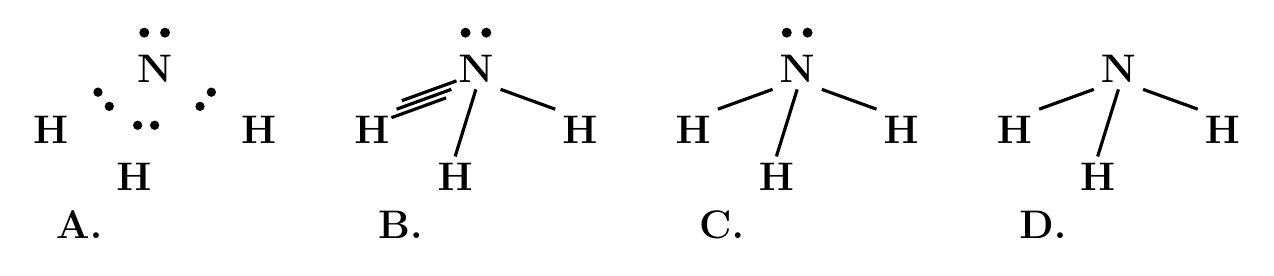
\begin{tikzpicture}[font=\bfseries\Large, line width=1.15pt, xscale=1.2, yscale=1.2]

% ==================== OPTION A ====================
\begin{scope}[shift={(0,0)}]
    \node[inner sep=2pt] (Na) at (0, 0.1) {N};
    \node[inner sep=2pt] (H1a) at (-1.1, -0.55) {H};
    \node[inner sep=2pt] (H2a) at (-0.22, -1.05) {H};
    \node[inner sep=2pt] (H3a) at (1.1, -0.55) {H};
    
    % Hai chấm trên đầu N
    \fill (-0.11, 0.48) circle (1.5pt);
    \fill ( 0.11, 0.48) circle (1.5pt);
    
    % Hai chấm giữa N và H bên trái (góc ~ 30 độ)
    \fill (-0.60, -0.15) circle (1.4pt);
    \fill (-0.48, -0.30) circle (1.4pt);
    
    % Hai chấm giữa N và H ở dưới (nằm ngang)
    \fill (-0.18, -0.50) circle (1.4pt);
    \fill ( 0.00, -0.50) circle (1.4pt);
    
    % Hai chấm giữa N và H bên phải (góc ~ -30 độ)
    \fill ( 0.60, -0.15) circle (1.4pt);
    \fill ( 0.48, -0.30) circle (1.4pt);
    
    \node[font=\bfseries\Large] at (-0.8, -1.55) {A.};
\end{scope}

% ==================== OPTION B ====================
\begin{scope}[shift={(3.4,0)}]
    \node[inner sep=2pt] (Nb) at (0, 0.1) {N};
    \node[inner sep=2pt] (H1b) at (-1.1, -0.55) {H};
    \node[inner sep=2pt] (H2b) at (-0.22, -1.05) {H};
    \node[inner sep=2pt] (H3b) at (1.1, -0.55) {H};
    
    % Hai chấm trên đầu N
    \fill (-0.11, 0.48) circle (1.5pt);
    \fill ( 0.11, 0.48) circle (1.5pt);
    
    % Liên kết ba N ≡ H1 (3 đường song song theo phương nối N-H1)
    % Vector từ Nb đến H1b có góc ~ -150 độ (pháp tuyến góc ~ 60 độ: dx = -sin, dy = cos)
    \draw ([shift={( 0.055, 0.09)}]Nb.south west) -- ([shift={( 0.055, 0.09)}]H1b.north east);
    \draw (Nb.south west) -- (H1b.north east);
    \draw ([shift={(-0.055,-0.09)}]Nb.south west) -- ([shift={(-0.055,-0.09)}]H1b.north east);
    
    % Liên kết đơn N - H2
    \draw (Nb.south) -- (H2b.north);
    
    % Liên kết đơn N - H3
    \draw (Nb.south east) -- (H3b.north west);
    
    \node[font=\bfseries\Large] at (-0.8, -1.55) {B.};
\end{scope}

% ==================== OPTION C ====================
\begin{scope}[shift={(6.8,0)}]
    \node[inner sep=2pt] (Nc) at (0, 0.1) {N};
    \node[inner sep=2pt] (H1c) at (-1.1, -0.55) {H};
    \node[inner sep=2pt] (H2c) at (-0.22, -1.05) {H};
    \node[inner sep=2pt] (H3c) at (1.1, -0.55) {H};
    
    % Hai chấm trên đầu N
    \fill (-0.11, 0.48) circle (1.5pt);
    \fill ( 0.11, 0.48) circle (1.5pt);
    
    % 3 liên kết đơn tỏa xuống
    \draw (Nc.south west) -- (H1c.north east);
    \draw (Nc.south) -- (H2c.north);
    \draw (Nc.south east) -- (H3c.north west);
    
    \node[font=\bfseries\Large] at (-0.8, -1.55) {C.};
\end{scope}

% ==================== OPTION D ====================
\begin{scope}[shift={(10.2,0)}]
    \node[inner sep=2pt] (Nd) at (0, 0.1) {N};
    \node[inner sep=2pt] (H1d) at (-1.1, -0.55) {H};
    \node[inner sep=2pt] (H2d) at (-0.22, -1.05) {H};
    \node[inner sep=2pt] (H3d) at (1.1, -0.55) {H};
    
    % 3 liên kết đơn (KHÔNG có hai chấm trên đầu)
    \draw (Nd.south west) -- (H1d.north east);
    \draw (Nd.south) -- (H2d.north);
    \draw (Nd.south east) -- (H3d.north west);
    
    \node[font=\bfseries\Large] at (-0.8, -1.55) {D.};
\end{scope}

\end{tikzpicture}
\end{document}
